\documentclass[a4paper,norsk]{article}
\usepackage[utf8]{inputenc}
\usepackage[T1]{fontenc,url}
\usepackage{babel,textcomp}
\usepackage{graphicx, wrapfig}
\usepackage{graphics}
\usepackage{amsmath}
\usepackage{stackengine}
\usepackage{listings}
\usepackage{amsfonts}
\urlstyle {sf}
\title {Project 2 in FYS-STK4155}
\author {Mikael Ravndal}
\begin{document}
\maketitle
\section{Abstract}
In this project we will take a look at classifying data using different methods from project 1 and neural networks. Can you predict all models with linear regression or can the neural networks ``black boxes''  solve problems which linear regression models cannot?

\section{The data}
\subsection{The 1D generated data}
In the 1D example we are interested in the J's of the nearest neighbor spins, which is multiplied to compute the energies. The energies are produced in the training data like this:
\begin{equation*}
  E[\hat{s}]=-J\sum_{j=1}^{N}s_{j}s_{j+1},
\end{equation*}
Here E is the energy and the s is the spins.\\
So the nearest neighbor interactions is what is used for the classifiers, not the actual spins itself.
\subsection{The 2D real data}
Now when I start to apply the methods on the 2D data, I will not compute the nearst neighbor interactions. I will instead use each spin as it's own parameter. This is, for my understanding, primarily because we are not interested in the computed J's anymore, but just interested in how the data produces the one's or the zero's.\\
Another reason is that if we computed the nearest neighbors interactions, we would have to compute a $(40x40)^2 = 256000$ line of numbers for each sample, which would end up with a huge amount of predictors.\\
This could result in a better prediction, but would take way more time to compute. So from a practical standpoint it is not a good idea to compute the interactions.

\clearpage
\section{Estimating the coupling constants of the Ising model using Linear regression}
We will now use our linear regression methods to estimate the values of J from the Ising model.\\
The training data was generated in the way that every $X_{i, i+1}$ was 1. So we are to expect a diagonal matrix for the coefficients where the values for every $X_{i, i+1}$ should be -1 and also the upper right corner should be one. The corner represents the interaction between the last and fist element.\\
Using Ordinary Least Squares we get these coefficients:\\
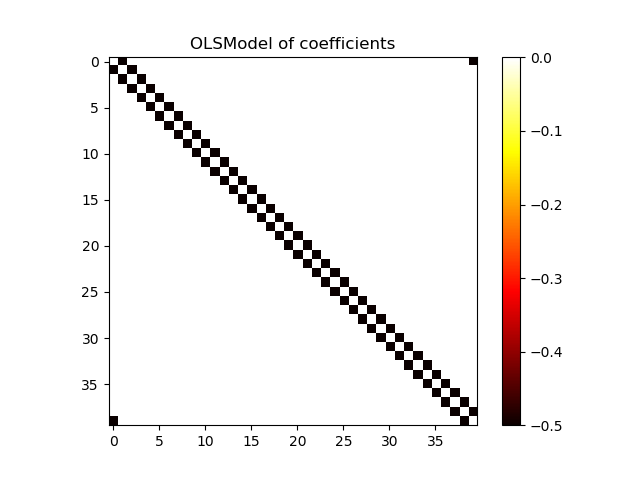
\includegraphics[scale=.7]{images/OLScoef}\\
We can tell that OLS can't tell that the interactions are from i to i+1 and not both ways. This doesn't do anything with the predictions, with the predictions the model is going to make. That's why it doesn't change this.


\subsection{Using Lasso and Ridge}
When we use the Lasso and Ridge methods we can play around with different values for $\alpha$ to see what fits best.\\
Looking at some Lasso models first:\\
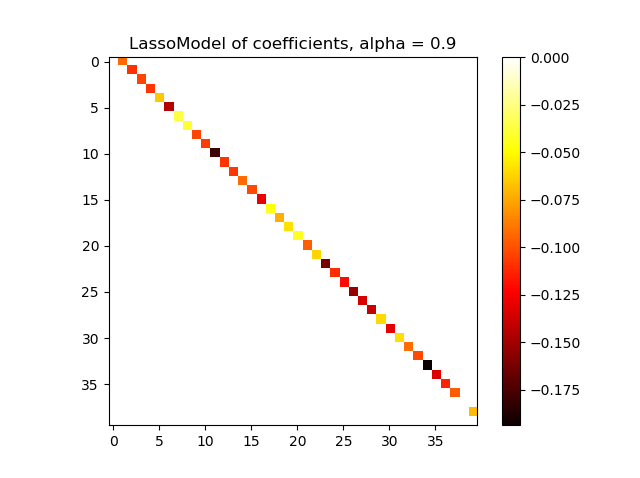
\includegraphics[scale=.7]{images/Lassocoef09}\\
R2: 0.18027321938745078, MSE: 34.97340045570735\\
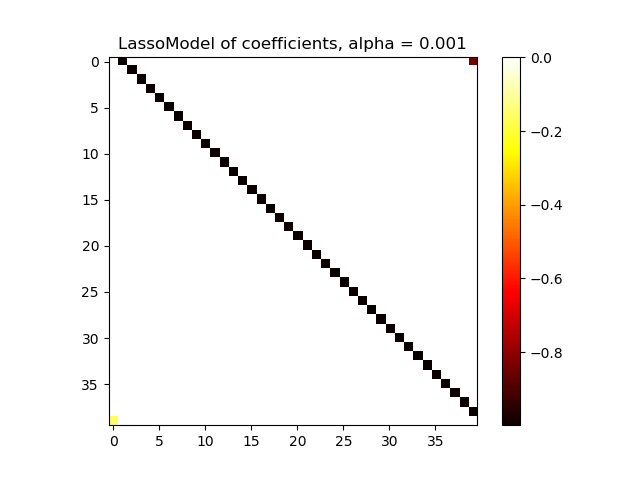
\includegraphics[scale=.7]{images/Lassocoef0001}\\
R2:0.9999989839436036, MSE: 4.33497453981647e-05\\
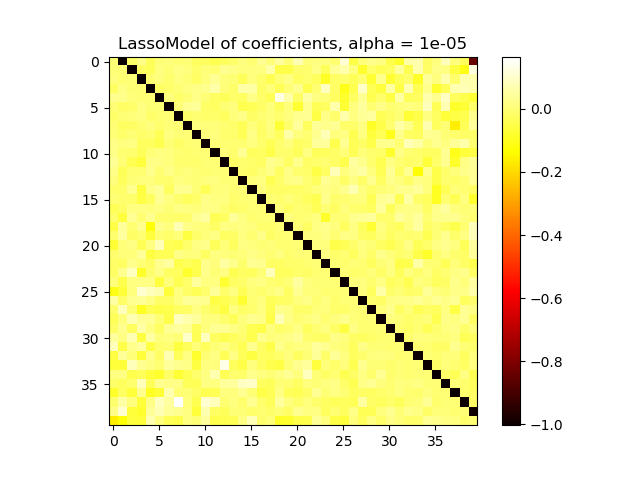
\includegraphics[scale=.7]{images/Lassocoef000001}\\
R2: 9999999981210006, MSE: 8.016695475884506e-08\\
\\
Taking a look at Lasso first, we can immediatly tell that this method actually predicts how our test data is generated. With a high $\alpha$ we can tell the predictions are weak, but on the right track. Lowering the $\alpha$ to 0.001, we can see that it predicts how the data was generated fairly well. There is only a little error in the connection between the first and last spin, but other than that it's a good prediction.\\
In the last image we see that all of the values for the betas rise up in the prediction. On first thought I would assume that this would affect the R2 and MSE-score negativaly, but since all of the values rises up, no single one dominates much more than the others. That's why the R2 and MSE-scores just get better, even though it doesn't match the generated data.\\
Let's look at a plot of the coefficients of the ridge model:\\
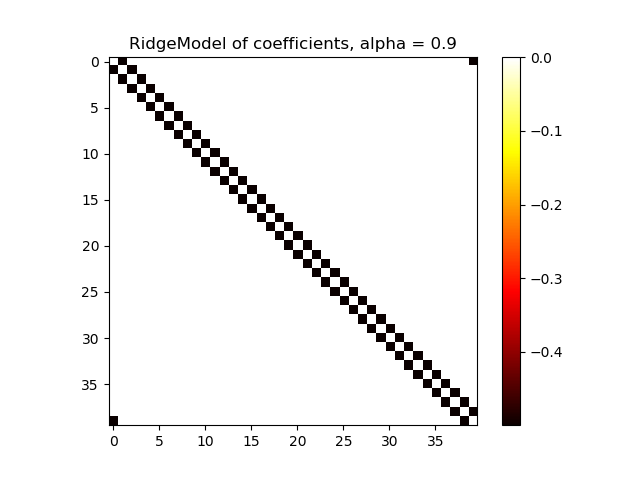
\includegraphics[scale=.7]{images/Ridgecoef09}\\
I have only include this image since the value of $\alpha$ doesn't seem to affect how Ridge behaves.\\
It behaves just like the ordinary least squares and the values for R2 and MSE are pretty low compared to Lasso with high $\alpha$:\\
R2 score of Ridge with alpha = 0.9\\
0.9999999971161928\\
MSE score of Ridge with alpha = 0.9\\
1.2303677455311343e-07\\
So in conclusion; Ridge and Lasso are both good in predicting this data, but Lasso does a more accurate job. Lasso accuartely predicts the exact J=1-values in the betas which we generated in the test data.


\subsection{Bias-variance analysis with bootstrapping}
Doing bootstrap on the data and computing the bias and variance. Data of different $\alpha$'s lies in the text file regression. We can take a look at the different models with $\alpha$ = 0.001. Data was as follows:\\
\\
Ridge:\\
alpha: 0.001000, bootstraps: 500\\
VAR: 37.649600\\
BIAS: 40.367488\\
\\
Lasso:\\
alpha: 0.001000, bootstraps: 500\\
VAR: 42.878464\\
BIAS: 40.222182\\
\\
The values are pretty even, but the variance of Ridge is approximately 10 percent lower. From the plots this makes sense, we saw a bit more variance in the betas in Lasso. Other than this both values are pretty even.\\
\\
From the theory we should expect a lower variance from Lasso, but this doesn't seem to be the case here. It seems like in this particular problem, Ridge eliminates the variance no matter the choice of alpha. Lasso solves the problem better, but is more vulnearable for the change in alpha.
\\
\section{Determing the phase of real data}
The next step is now to look at real two dimensional data and try to classify them using logistic regression. The data we are looking at looks like this:\\
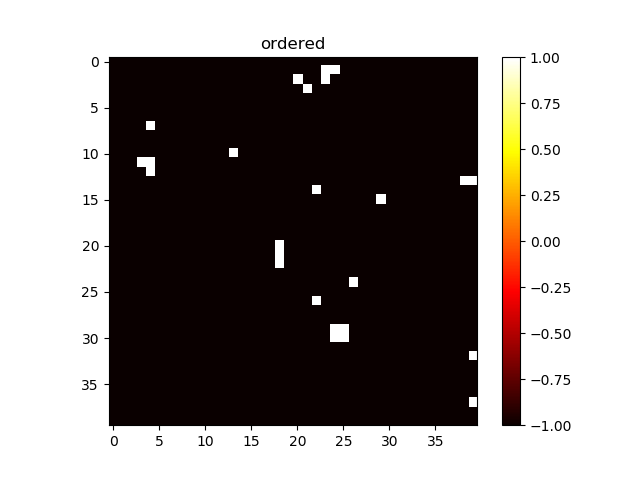
\includegraphics[scale=.7]{images/ordered}\\
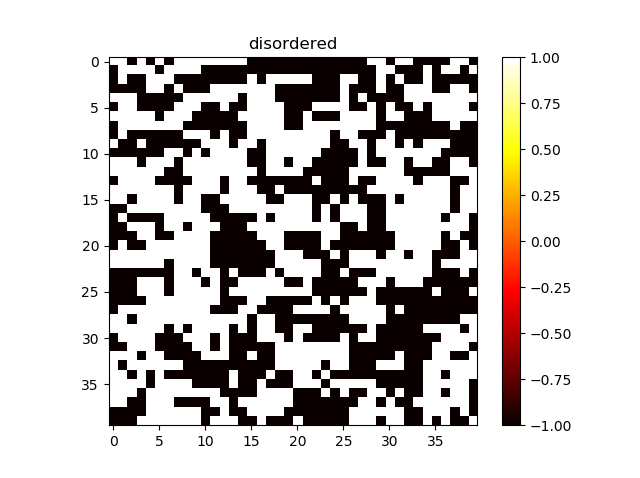
\includegraphics[scale=.7]{images/disordered}\\
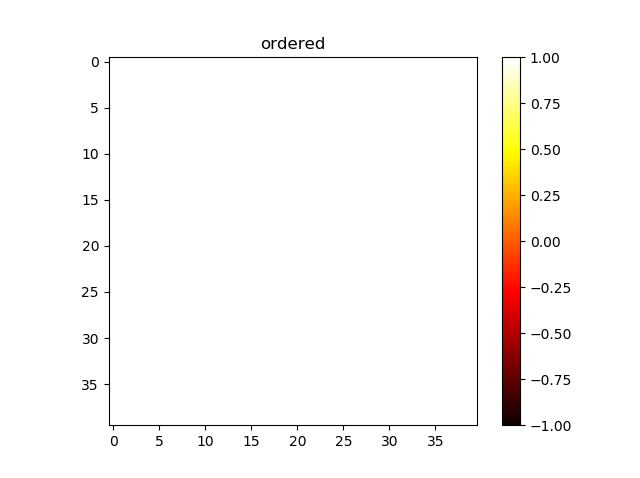
\includegraphics[scale=.7]{images/orderedv2}\\
We can get an intuitive feel of what it means for it to be ordered and disordered. If there is a big mix in the data, then it is disordered. If not, it is ordered.

\subsection{Logistic regression}
My algorithm will use the gradient descent method. This is an iterative process where we calculate new betas for each iteration by the algorithm:
$$
\beta_{k+1} = \beta_{k} - \gamma \nabla_{\beta} C(\beta_{k}) \qquad,k = 0, 1, ...
$$
Here $\gamma$ is the step size, which is set to a relatively small number; 0.0001. $\nabla_{\beta} C(\beta_{k})$ is the derivative of the cost function of the problem which is defined as:
$$
C(\beta) = || X\beta - y ||^2 = ||X\beta||^2 - 2y^T X \beta + ||y||^2
$$
Then we compute the derivative over each beta and get:
$$
\nabla_\beta C(\beta) = 2 X^T (X\beta - y)
$$
Then this gets computed over each epoch and we step closer to the correct solution.
By modifying the existing code in how to implement the data, we can use logistic regression on it.\\
\\
This is the gradient descent method, but in my case I am using stochastic gradient descent.\\
The underlying idea comes from that you can write $ C(\beta) = \sum^{n}_{i=1} c_i (x_i, \beta)$. Using this we it follows that the derivative can be written as:
$$\nabla_\beta C_n (\beta) = 2 {X_ n}^T ({X_n}\beta - y_n)$$
where n determines how many samples we choose. This will make calculations go much faster. The downside is the element of randomness: We will not get the same fit each time. That's why it's being runned several times. We should, however, expect similar results each time, because we run over so many iterations.\\
\\
Using scikitlearn's methods we get a accuracy score of 0.7053117408906883 when training to test ratio is 0.95. This might seem like a decently high number, but this accuracy is closer to 50 percent than it is to a 100 percent.\\
If we try to compare it a bit to the linear regression scores, they got mostly an R2-score of 0.99 or higher. Even if you can't compare the different methods directly, a .99 score in R2 is an almost perfect score.\\
An accuracy score of 0.70 is closer to guessing than it is to predicting accurately.\\
After running a lot of tests we can tell that our stochastic gradient descent model mostly gets an accuracy score around .70. It is a little inconsistent with scores of 0.50 and 0.90, but mostly it gets to a score of 0.70. We can tell if we run the algorithm with an max iteration of 1000 it tends to overfit, so the accuracy gets lower.\\
After cutting down on tests-samples and looking at the plot of the accuracy score using different parameters, we arrive at a couple of different conclusion.\\
First let's look at how the accuracy score changed over 1000 iterations:\\
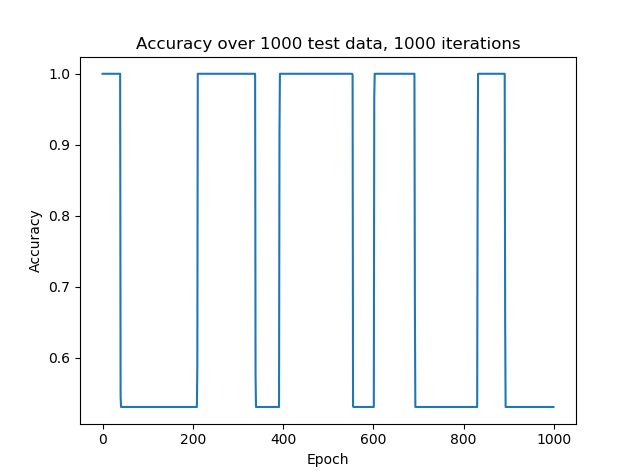
\includegraphics[scale=.7]{images/logplots/1000iter1}\\
It seems like the method is switching between two local optimums, where one of them is clearly better than the other one. This is done with a low eta and it turns out this way no matter the choice of etas that I've tried. If we run it one more time, we get these accuracies:\\
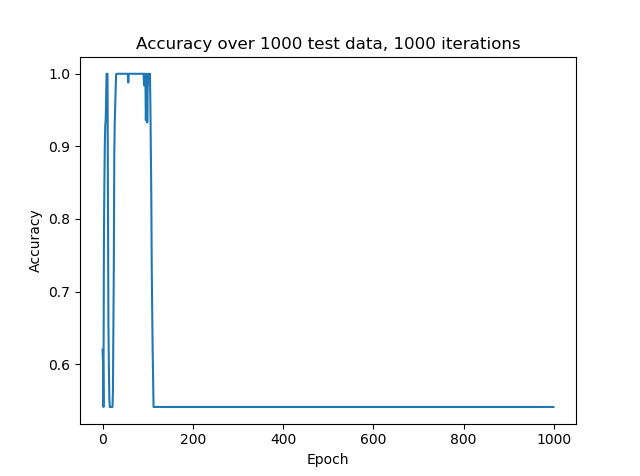
\includegraphics[scale=.7]{images/logplots/1000iter2}\\
So we can tell that these local optima, definitely are there and it didn't get out of the poor local one.




\clearpage
\section{Regression of one-dim Ising model using neural network}
\subsection{Quick visual}
Here is an image of how I modelled the neural networks. Both networks are multilayered perceptrons, with 150 hidden nodes. We then have 1600 as the input layer, each of the spins. In the output layer there is only one layer, the predicted energy.\\
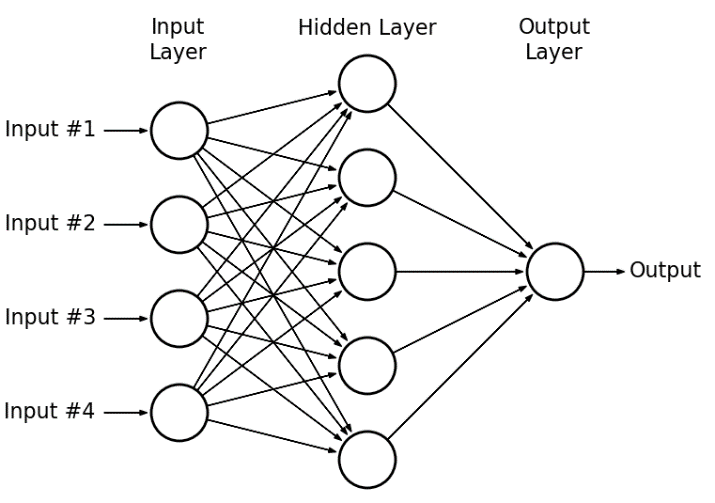
\includegraphics[scale=.4]{images/mlplayout}\\
\subsection{Using a neural network}
Now we will take a look at neural networks to see if they can solve what we made the linear regression models solve. Testing around a bit with Tensorflow I figured out that a multi layered perceptron with 150 nodes in the hidden layer would work just fine.\\
We are using the backpropagation algorithm to adapt the weights in the network.\\
The function which is used in the hidden nodes are the sigmoid function and use a linear function in the output node.\\
Using a linear function makes it able to guess numbers along the real axis, instead of numbers between zero and one.
The train-algorithm of the network calclulates the R2-score over the test-data between every iteration/generation. This is stored and we can look at the plot how well it does over 100 iterations/generations.\\
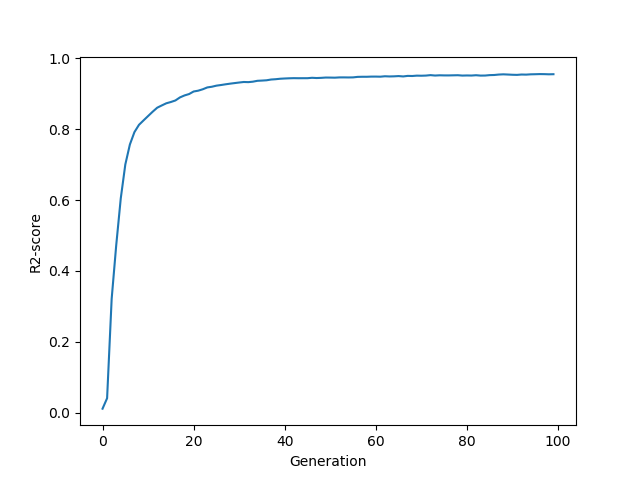
\includegraphics[scale=.7]{images/linearNN}\\
We can tell that it converges to an R2-score of approxematily 0.95, which is very acceptable.\\
Doing the same with TensorFlow gave an R2-score of 0.9894. So it is a pretty solid R2-score, but the linear regression actual does it better.\\
Taking a look at some predictions to see how it does:\\
\begin{center}
    \begin{tabular}{| l | l | l | l |}
    \hline
    Sample \# & My NN & TF NN & Actual data \\ \hline
    172 & 3.76808941 & 4.386107 & 4. \\ \hline
    583 & -6.95956579 & -8.253661 &-8. \\ \hline
    787 & 9.37251406 & 8.00584 &8. \\ \hline
    850 & -0.01350432 & 0.55443907 &0. \\ \hline
    481 & 4.84370393 & 4.3612957 &4. \\
    \hline
    \end{tabular}
\end{center}
The R2-score tells us of course most of how accurate it is, but it is nice to have some examples on how the neural network does.\\

\clearpage
\section{Classifying the Ising model phase using neural networks}
Now we have to change up the neural networks cost-function. Following this we also have to change at least the function in the outputnode.\\
What I did is I continued using the sigmoid function in the hidden layer. After this, we change the output function to be sigmoid. This felt the most natural and we get pretty good results fast.\\
Here is a plot of how the accuracy behaved in the span of the epochs:\\
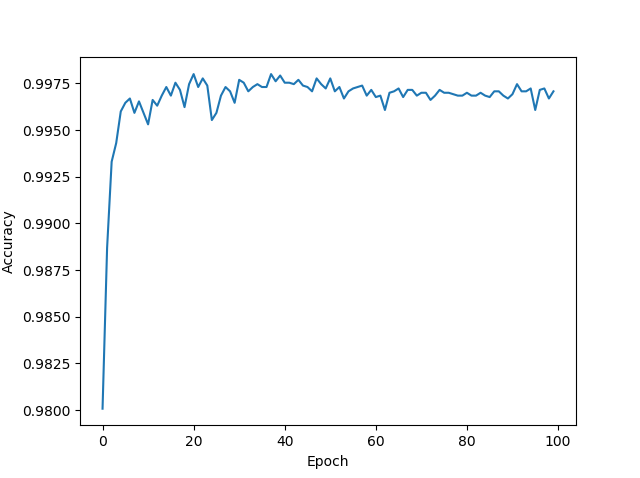
\includegraphics[scale=.7]{images/classNN100epoch}\\
It ends up with an accuracy of 0.997 which is extremely good. This means that we can rely on our neural network. For every 1000th prediction, it will only guess wrong 3 times.\\
This is great numbers, but TensorFlow has again better scores. During training it actually had a 100\% correct prediction accuracy. It ended up with an accuracy score of 0.9999230769230769. So this neural net gets every 13000th prediction wrong. 



\clearpage
\section{Evaluation of the different methods}
\subsection{Regression}
There is a lot of parameters to tweak in the regression method and there is a lot of activation functions, different layers and maybe different numbers in the output layer. I have not experimented that much with all of the parameters, but the regression methods seems to hold up better than the neural networks. We can take a look at this image of how lasso very accurately predicted the J's in the generating of the data:\\
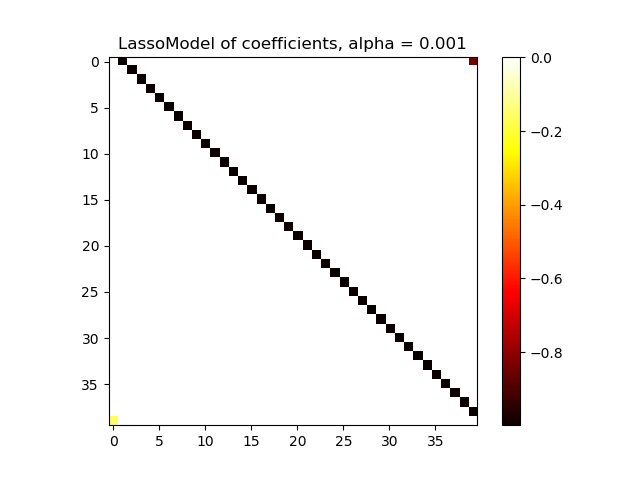
\includegraphics[scale=.7]{images/Lassocoef0001}\\
The positive thing with this compared to the neural network is that we are able to take a look into the ``black box '' which is the betas. This gives us as interpreders of the methods a better understanding of what is actually going on. Even though the neural network did well and could possibly done better than the regression with more hidden layers and different activation functions, we would not get the same grasp of what is actually going on. We get this out of the regression methods, which is a positive thing.\\
\\
So for this exact problem, I would choose Lasso with an alpha = 0.001, just like the picture.
\subsection{Classification}
The logistic regression method has a lot of variance in it when we fit it some times, but overall it seemed to land at an accuracy score of 0.70. This is very poor, so these models wouldn't be acceptable for classifying futere data. It is worth noticing that we didn't use the nearest neighbor interactions as the input. We just used the spins on it's own. This might affect how the logistic regression does and calculating the spins might have resulted in better predictions. This would however take a lot of data points for each sample, which would take a very long time to compute. Each sample would be of size $1600^2$ compared to just $1600$. But I am quite confident that we would get better predictions using the interactions. The reason being that from the 1D data, we got extremely good prediction from the Lasso model. So using more predictors with the logistic regression should result in better predictions.\\
\\
On the other hand, the neural networks did extremely well here. I only ended up using the mult layered perceptron, but it did just fine. Maybe more layers and mixing it up with different activation functions would have resultet in even better outcomes. The reason why I think it worked in this case is that a neural network is more prone to classify on the interactions between the inputs. So the interactions between the inputs gets taken care of, through how the neural network's layout is. Since there originally isn't a ton of interactions to take care of, the multi layered perceptron does just fine in classifying.\\
TensorFlow's network got sometimes a whopping 100\% accuracy score at times, even when it was tested on all of the test samples.\\
\\
My conclusion here is to use the neural network. It would be fine using regression methods, but I think it needs to much pre-computing of the already existing data. If it is not that important to know how our method classifies, it is definitely wiser to use the neural network.

\section*{Referances}
\begin{enumerate}
  \item Hastie, Trevor, Tibshirani, Robert, Friedman, and Jerome. \textit{The Elements of
Statistical Learning}. Springer, 2009.
  \item Ravndal and Baar. Project 1, fys-stk4155, 2018.
  \item Ravndal. Project 2, fys-stk4155, 2018.
  \item Michael Nielsen. How the backpropagation algorithm works. 2018
\end{enumerate}


\end{document}
